\section{Introduction} \label{introduction}
%% General Introduction
In machine learning applications, a pipeline, a series of complex data processing steps, processes a labeled training dataset and produces a machine learning model.
The machine learning model is then used to make predictions on new unlabeled data.
The model then has to be deployed into a deployment platform where it can answer prediction queries in real-time.
To properly preprocess the prediction queries, typically the pipeline has to be deployed alongside the model.

%% Intro to the problem of continuous improvement
After the model is deployed, new training data may become available.
Typically, the deployment platform utilizes online learning methods to further train the deployed model.
In online learning, the model is updated based on the incoming data points.
Online learning can adapt the model to the new training data and provide an up-to-date model.
However, updating a model using individual data points may introduce instability and is not always effective.
In some applications that online learning has proven to be effective, to guarantee the same level of quality as the offline batch training, one has to tune the online learning method to the specific use case \cite{ma2009identifying, macmahan2013}.
Therefore, to solve the problem of low model quality, the deployment platform performs periodical offline batch retraining over the existing historical and newly available data.

Figure \ref{fig:motivational-example} shows the typical process of the existing deployment platforms.
During the initial training step, a user designs a machine learning pipeline that consists of several data and feature preprocessing steps and trains a machine learning model by utilizing a batch training algorithm.
Then in the deployment step, the model and the pipeline are deployed into the deployment platform.
To perform inference, the deployment platform directs the incoming prediction queries through the preprocessing steps.
Using the preprocessed features, the model makes a prediction.
During the online update phase, the deployment platform directs the data through the preprocessing steps of the pipeline and then, using an online training algorithm, the platform updates the model.
Finally, the deployment platform accommodates periodical retraining of the pipeline by either automatically initiating a batch training or prompting the user to train and redeploy a new model to the deployment platform.
During the periodical retraining, the deployment platform has to disable the online updating of the model.

One of the challenges in many real-world use cases is the size of the training datasets.
Typically, training datasets are extremely large and require hours or days of data preprocessing and training to result in a new model.
Therefore, it is not feasible to train a new model frequently.
But in some applications, retraining the model is critical, as even a small increase in the quality of the deployed model can have a large financial impact.
For example, in the domain of ads click-through rate (CTR) prediction, even a 0.1\% accuracy improvement yields hundreds of millions of dollars in revenue \cite{ling2017model}.

Despite the very high training cost, the periodical retraining deployment approach has two advantages.
First, the tuning process is very simple.
A user only has to define one parameter for how often the deployment platform should retrain a new model.
Second, the deployment platform can accommodate a wide range of machine learning models and pipelines.

Therefore, an efficient and robust deployment platform must have three important characteristics.
First, it must be able to maintain the quality of the deployed models without incurring a high training cost.
Second, the platform must be easy to tune.
Finally, the platform must accommodate different types of machine learning models and pipelines.
We propose a deployment platform, that completely eliminates the need for retraining, thus greatly reducing the training cost, while achieving the same level of quality that a deployment platform with periodical retraining of the models would achieve.
Our deployment platform is robust and accommodates many different types of machine learning models and pipeline components.
Moreover, the tuning process is the same as the periodical retraining deployment approach.

%% Use case
\begin{figure}[h!]
\centering
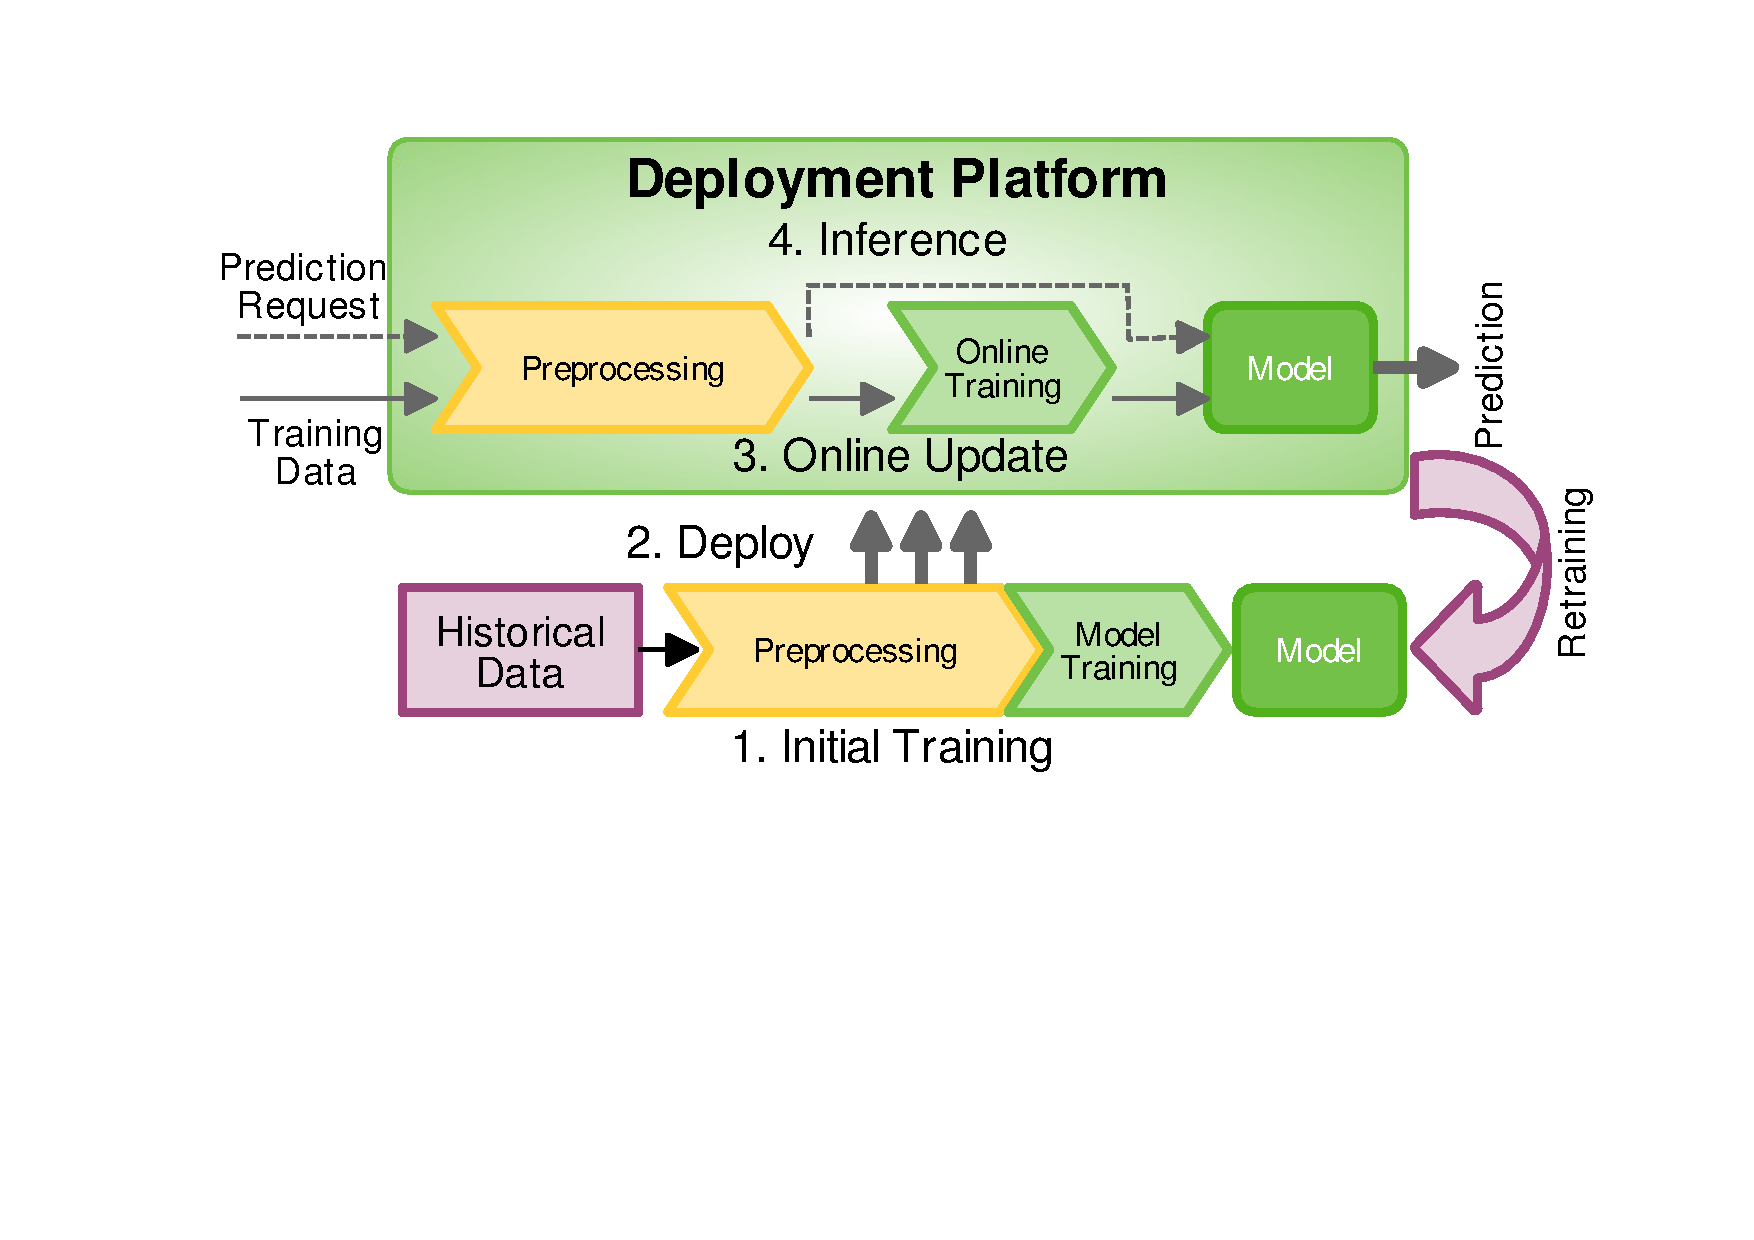
\includegraphics[width=\columnwidth]{../images/generic-motivational-example-v2.pdf}
\caption{Deployment process of machine learning pipelines}
\label{fig:motivational-example}
\end{figure}

%One example is the problem of Ad click prediction \cite{macmahan2013}.
%In Ad click prediction, the machine learning pipeline consists of extracting features from the users and ads. 
%Logistic regression models perform well in this setting \cite{macmahan2013}.
%Prediction queries consist of the user's information and a pool of available ads for displaying to the user.
%Once a prediction is made, a set of ads, with highest prediction scores, are displayed to the user.
%Based on the action of the user (click or no click), new training data will be generated which is sent to the deployment platform for further training of the model.
%Aside from the generated training data, new ads and new users are constantly becoming available.
%As a result, new models have to be periodically trained and redeployed into the deployment platform.

%The above example demonstrates the complexity and suboptimality of the deployment and maintenance of machine learning models and pipelines through periodical retraining.
%Therefore, a flexible deployment platform should meet the model quality requirement without requiring the periodical retraining of the models and pipelines.

%% Our solution
Our deployment platform continuously updates the model using a combination of the historical and incoming training data.
Similar to existing deployment platforms, our platform also utilizes online learning methods to update the model based on the incoming training data.
However, instead of periodical retraining, our deployment platform performs regular updates to the model based on samples of the historical data.

Our deployment platform offers two key optimizations, proactive training and online statistics computation and feature materialization. 

\textit{Proactive training.}
Proactive training is the process of utilizing samples of the historical data to update the deployed model.
First, the deployment platform processes a given sample using the pipeline, then it computes a partial gradient and updates the deployed model based on the partial gradient.
The updated model is immediately ready for answering prediction queries.
Unlike periodical retraining, each proactive training is very fast (similar to one iteration of offline training) and does not require the deployment platform to disable the online update.
Our experiments show that proactive training of the model achieves a similar or even a lower error rate over time and reduces the training time by an order of magnitude when compared to the periodical deployment approach.

\textit{Online Statistics Computation and Feature Materialization.}
Before updating the model using proactive training, the pipeline has to process the training data.
Every component of the pipeline needs to scan the data, updates the statistics (for example the mean and standard deviation of the standard scaler component), and finally transform the data.
Computing these statistics and transforming the data are time consuming processes.
Aside from the proactive training, our deployment platform also employs online learning methods to update the model in real-time.
During the online training, the deployment platform has to direct the data through the pipeline before updating the model.
During the online learning, we compute the required statistics and transform the data.
The deployment platform stores the updated statistics for every pipeline component and materializes the transformed features by storing them in memory or disk.
By reusing the computed statistics and the materialized features during the proactive training, we eliminate the data preprocessing steps of the pipeline and further decrease the proactive training time.

% Our contributions
In summary, our contributions are:
\begin{itemize}
\item A framework for continuously training deployed machine learning models and pipelines that adapts to the changes in the incoming data. The framework accommodates different types of machine learning models and pipelines. In our experiments, we design and deploy three different machine learning pipelines.
\item Proactive training of the deployed models and pipelines that frequently updates the model in-place using a combination of the historical and the incoming data which guarantees high-quality models while completely eliminating the periodical retraining of the deployed model.
\item Efficient pipeline processing and model training by online statistics computation and feature materialization, thus guaranteeing the availability of up-to-date models for answering prediction queries.
\end{itemize}

The rest of this paper is organized as follows:
Section \ref{continuous-training-serving} describes the details of our continuous training approach.
In Section \ref{sec:system-architecture}, we introduce the architecture of our deployment framework.
In Section \ref{evaluation}, we evaluate the performance of our continuous deployment approach.
Section \ref {related-work} discusses the related work.
Finally, Section \ref{conclusion} presents our conclusion and the future work.